\chapter{Implementierung} \label{chap:Implementierung}
\thispagestyle{empty}
In diesem Kapitel werden die implementierten Funktionen und Klassen dokumentiert. Dabei wird zunächst der Aufbau und Ablauf von klassenbasierten Unit-Tests aus dem MATLAB\textsuperscript{\textregistered} Unit Test Framework beschrieben und wie sich damit ein Konzept für das szenariobasierte Testen realisieren lässt. Weiterhin werden die implementierten Szenarien sowie deren Parametrierung und Ergebnisbewertung durch KPIs vorgestellt und auf ausgewählte Szenarien näher eingegangen. Abschließend wird die Implementierung in der Gitlab CI Pipeline erläutert.

\section{Anforderungen} \label{sec:Anforderungen}
Aus der Aufgabenstellung ergeben sich bereits die wichtigsten Anforderungen. Zunächst soll ein Konzept für das Testen der MPFC basierend auf dem MATLAB\textsuperscript{\textregistered} Unit Test Framework erarbeitet werden. Dafür muss eine geeignete Struktur gefunden werden, welche eine automatisierte Ausführung ermöglicht und Variationen von sowohl Testparametern (bspw. Initialgeschwindigkeiten) als auch MPC-Parametern (bspw. Gewichte der Kostenfunktion) leicht umzusetzen sind. 

Es sollen Szenarien gefunden und parametriert werden, welche für den Regelungsalgorithmus eine Herausforderung darstellen und so das Verhalten in kritischen Situationen getestet werden kann.

Um die Simulationsergebnisse bewerten zu können, sollen geeignete Kriterien festgelegt werden, die sowohl Sicherheit als auch Komfort der gefundenen Lösung bewerten. Aus den Testergebnissen soll ein Bericht erstellt werden, welcher dem Entwickler übersichtlich mögliche Fehlschläge aufzeigt.

\section{Simulationsumgebung} \label{sec:Simulationsumgebung}
Die Simulationsumgebung und der Regelungsalgorithmus sind bereits in vorherigen Entwicklungsprojekten bei der IAV entstanden und sind in MATLAB\textsuperscript{\textregistered}/Simulink implementiert. Aus den Streckeninformationen wird ein gewünschter Pfad mit einer Zielgeschwindigkeit generiert. Abbildung \ref{fig:Simulation_Strecke} zeigt den generierte Live-Plot, welcher bei Start der Simulation das Fahrzeug auf der Strecke darstellt.
\begin{figure}[ht]
    \centering
    \includegraphics[width=0.6\textwidth]{figures/3_Implementierung/simulationsumgebung.pdf}
    \caption{Beispiel einer komplexen Simulationsstrecke}
    \label{fig:Simulation_Strecke}
\end{figure}

\section{MATLAB\textsuperscript{\textregistered} Unit Test Framework} \label{sec:MatlabUnitTest}
MATLAB\textsuperscript{\textregistered}, in der für dieses Praktikum verwendeten Version 2022a und 2023b, stellt in der Basiskonfiguration ein umfangreiches Framework für die Implementierung von Unit Tests zur Verfügung \cite{matlabTest}. Eine Verwendung dieser Funktionalität für das Testen der MPFC liegt nahe, da diese vollständig in diesem Programm implementiert ist.

Grundsätzlich gibt es drei Arten von Testabläufen: skriptbasierte, funktionsbasierte und klassenbasierte Tests. Nach Befassen mit den entsprechenden Dokumentationsseiten wurde sich für die Nutzung der klassenbasierten Tests entschieden, da diese den größten Funktionsumfang bieten. Ein entscheidender Faktor ist die Möglichkeit, Tests durch externe Parameter zu parametrieren, was eine direkte Anforderung an das zu entwickelnde Konzept ist \cite{matlabTest}.

Das von Mathworks implementierte Framework ähnelt in vielen Gesichtspunkten der xUnit Architektur indem es die gleichen grundlegenden Strukturen aufweist \cite{xUnitWiki}. Die kleinste Einheit dieser Architektur ist der \textit{test case}. In diesem wird über \textit{assertions}, dies sind meist logische Operationen, festgestellt, ob sich ein System im Normbereich verhält. Ist dies nicht der Fall, wird der Test abgebrochen und als fehlgeschlagen angesehen.

Um sicherzustellen, dass sich das \textit{System Under Test (SUT)} vor einem Test in einem definierten Zustand befindet und vorherige Programmausführungen keine Auswirkungen auf die Testergebnisse haben wird über \textit{test fixtures} dieser definierte Zustand hergestellt \cite{xUnitpatterns}. Bei klassenbasierten Tests gibt es mehrere Stellen an denen initiale Zustände hergestellt werden können. Mithilfe der Setup-Methoden können Voraussetzungen für mehrere Klassen (shared fixtures), für alle Testfälle einer Klasse (testclass setup) initial oder vor Ausführung jedes einzelnen Testfalls (testmethod setup) geschaffen werden.

Eine \textit{test suite} ist eine Sammlung von Testfällen, welche die gleichen Initialzustände teilen. Da in der späteren Implementierung eine Testsuite immer aus lediglich einer Testklasse erstellt wird bezeichnen Testsuite und Testklasse hier das gleiche Objekt. 

Bei klassenbasierten Tests ist es möglich, externe Parameter in die Testklasse zu laden. Diese können als Testparameter, Testinitialisierungsparameter oder Klasseninitialisierungsparameter übergeben werden. Abhängig davon, welche Parametertypen und wieviel Variationen definiert sind, werden Testfälle und die verschiedenen Setup-Methoden mehrmals ausgeführt. Eine eigene Darstellung des Ablaufs einer Testklasse ist in Abbildung \ref{fig:Testklassen_Ablauf} zu sehen. 

\begin{figure}[ht]
    \centering
    \includegraphics[width=0.75\textwidth]{figures/3_Implementierung/Testklassen_Ablauf.drawio.pdf}
    \caption{Ablauf von klassenbasierten Tests}
    \label{fig:Testklassen_Ablauf}
\end{figure}

Ein konfigurierbarer \textit{test runner} führt die Tests aus. Das Framework sorgt selbstständig dafür, dass die notwendigen Setup-Methoden an den richtigen Stellen ausgeführt werden.

Für die Darstellung der Testergebnisse existiert ein \textit{test result formatter}, welcher die Ergebnisse in vielen Formaten, beispielsweise PDF order XML, aufbereitet.

Die objektorientierte Natur von MATLAB\textsuperscript{\textregistered} und dem Unit Test Framework ermöglichen zusätzlich die Erweiterung der Funktionalität durch das Schreiben von eigenen oder Erweiterung von vorhandenen Plugins.

\section{Aufbau und Ablauf eines Szenarios} \label{sec:AufbauSzenario}

Nachdem die Funktionalitäten des Unit Test Frameworks erfasst wurden kann eine geeignete Implementierung basierend auf den Anforderungen erfolgen. Ein Szenario wird in der Simulation durch das Laden von entsprechenden Parametern bzw. Variablen definiert. Beim Starten der Simulation werden diese in das Simulink Modell geladen. Über die Protokolllierungsfunktion von Simulink werden die Simulationsergebnisse erfasst und für die weitere Verarbeitung abgespeichert.

\subsection{Simulationsparameter}
Zur vollständigen Beschreibung eines Szenarios werden initial folgende Parametersätze bzw. Variablen benötigt:
\begin{itemize}
	\item Fahrzeugparameter
	\item Initialzustände
	\item MPC Parameter
	\item Streckeninformationen
	\item (nur für ACC) Objekttrajektorie
\end{itemize}
Die Fahrzeugparameter, wie zum Beispiel die Länge eines Fahrzeugs oder die Parameter für das Fahrzeugmodell, gehen aus der betriebsinternen Dokumentation hervor. Diese werden über ein Skript geladen und sind fahrzeugspezifisch. Der Parameter hier ist lediglich das verwendete Fahrzeug.

Der Initialzustand eines Fahrzeugs kann mehrere Parameter umfassen. Hier kann beispielsweise die Geschwindigkeit zu Beginn der Simulation oder ein Versatz zum gewünschten Pfad vorgegeben werden.

Die MPFC wurde durch geeignet Methoden, beispielsweise wie in \cite{math11020465} vorgestellt, für die gestellten Anforderungen der Fahrzeugführung parametriert. Es stehen für verschiedene Fahrweisen, von komfortabel bis sportlich, Parametersets zur Verfügung. Das gewählte Parameterset ist damit ein weiterer Simulationsparameter.

Nachdem Fahrzeug und Regler initialisiert sind, wird im nächsten Schritt ein zu folgender Pfad generiert. Dafür steht eine Bibliothek zur Verfügung, mit deren Hilfe ein Pfad aus einfachen geometrischen Objekten - Gerade, Kreisbogen und Klothoid - erzeugt werden kann. Eine Klothoide ist ein Kreisbogen, dessen Krümmung proportional zur Länge ist und somit keinen Sprung in der Krümmung aufweist \cite{klothoidWiki}.

Für Szenarien, welche die Funktionalität der MPFC als Abstandsregeltempomat (Adaptive Cruise Control - ACC) testen wird zusätzlich die Trajektorie des vorausfahrenden Fahrzeugs benötigt.

\subsection{Ablauf eines Testskripts} \label{subsec:Testskript}
Ein Testskript vereint die korrekte Initialisierung der Simulation durch Ausführung entsprechender Skripte, Erstellen einer Testsuite aus einer Testklasse und Parameterwerten, Ausführung der Testklasse bzw. Simulation und die Erstellung von Testberichten. Der schematische Ablauf ist in Abbildung \ref{fig:Testskript_Ablauf} dargestellt.\medskip

\noindent Für den Start eines Szenarios wird der Codename für das Szenario und das zu verwendende Fahrzeug benötigt. Nach Ausführung von Initialisierungsskripten werden Parametersätze generiert, worauf in \ref{subsec:Parametergenerierung} näher eingegangen wird. Als nächstes wird aus einer Umgebungsklasse eine neue Instanz geschaffen. In dieser wird eine Testsuite erstellt. Wie in \ref{sec:MatlabUnitTest} bereits erwähnt besteht eine Testsuite immer aus einer Testklasse. Eine Testklasse implementiert ein Szenario, indem es die benötigten Variablen korrekt lädt, die Simulation ausführt und die Simulationsergebnisse in ihren Testfällen bewertet. Bei der Erstellung der Testsuite werden die vorher generierten Parameter in die Testklasse geladen.\medskip

\noindent Der konfigurierte Testrunner kann nun die Testsuite ausführen. Dabei werden die teilweise szenarien- und parameterabhängigen KPIs für die Bewertung der Simulationsergebnisse geladen. In \ref{subsec:KPI} wird darauf näher eingegangen.\medskip

\noindent Aus den Ergbenisse der Tests wird schließlich automatisiert ein Testbericht in PDF-Format für den Entwickler und in XML-Format für die Darstellung in der CI Pipeline, siehe \ref{sec:CIPipeline}, generiert.

\begin{figure}[ht]
    \centering
    \includegraphics[width=0.9\textwidth]{figures/3_Implementierung/Ablauf_TestSkript.drawio.pdf}
    \caption{schematischer Ablauf eines Testskripts zur Ausführung eines Szenarios}
    \label{fig:Testskript_Ablauf}
\end{figure}

\subsection{Parametergenerierung} \label{subsec:Parametergenerierung}
In bisherigen Testdurchführungen wurden die Parameter für Szenarien manuell gewählt und in ein Skript geschrieben. Für eine größere Anzahl an Parametern bzw. eine größere Testabdeckung ist dieses Verfahren sehr aufwändig und deckt möglicherweise nicht den gesamten Parameterraum ab. Wie bereits in Kapitel \ref{sec:SoftwaretestsAutomobil} geschildert ist es nicht möglich jede Parameterkombination eines ausgewählten Szenarios abzutesten. Besitzt ein Szenario $N$ Parameter und exisitieren für jeden dieser Parameter $k$ verschiedene Werte so werden bei einer vollständigen Abtestung des Parameterraums $k^{N}$ Simulationen benötigt. Die Anzahl der Simulationen steigt exponentiell mit der Anzahl der Parameter an. Vorallem bei komplexeren Szenarien ist diese Parametrierungsstrategie nicht anwendbar.

Um die Anzahl der notwendigen Simulationen zu reduzieren wurden folgende Strategien angewendet:
\begin{itemize}
    \item sinnvolle Begrenzung des Parameterraums
    \item Implementierung einer (zufälligen) Sampling Methode
    \item Diskretisierung des Parameterraums
\end{itemize}
Die Begrenzung des Parameterraums geschieht durch festlegen von Ober- und Untergrenzen für Parameterwerte. Diese Grenzen können durch das verwendete Fahrzeug gegeben sein, beispielsweise minimale Lenkradien oder Höchstgeschwindigkeiten oder durch Normen festgelegt. Beispielsweise werden in \cite{Bau2019} minimale Kurvenradien bei der Anlage von Straßen beschrieben. Noch fehlende Parametergrenzen wurden durch Testen der Funktionen der aktuellen MPFC Implementierung sinnvoll festgelegt.

Die Implementierung einer Sampling Methode, wie zum Beispiel dem Monte-Carlo-Verfahren, ermöglicht eine Reduzierung der Anzahl der benötigten Simulationen. Für jeden Parameter wird aus dem jeweiligen Parameterraum ein zufälliger Wert gezogen. Dies wird für eine vorher definerte Anzahl an Samples wiederholt.

Es kann allerdings nicht gewährleistet werden, dass der gesamte Parameterraum abgedeckt wird. Deshalb wird in der Implementierung das Latin Hypercube Sampling (LHS) angewendet, welches eine bessere Verteilung der Samples im Parameterraum gewährleistet, wie in Abbildung \ref{fig:Random_vs_LHS} dargestellt ist. Grundidee hierbei ist, dass jeder Parameterraum in $k$ Teilintervalle unterteilt wird. Es werden $k$ Samplesets generiert. Aus jedem Teilintervall wird dabei immer genau ein Wert zufällig gezogen, sodass nach Abschluss der gesamte Parameterraum abgedeckt ist. Aufgrund der zufälligen Ziehung innerhalb eines Intervalls ist das LHS dennoch eine Monte-Carlo Methode \cite{McKay1979}.\bigskip

\noindent Nach Ausführung dieser Funktion entstehen $k$-Samplesets, die für alle Parameter in den jeweiligen Grenzen eine gute Abdeckung des Parameterraums bieten.

\begin{figure}[ht]
    \centering
    \includegraphics[width=0.5\textwidth]{figures/3_Implementierung/LHS_random_compare.png}
    \caption{Vergleich der Verteilung von zufälligen Sampling mit Latin Hypercube Sampling \cite{Preece2015}}
    \label{fig:Random_vs_LHS}
\end{figure}

\subsection{Definition von Key Performance Indicators und Testkriterien} \label{subsec:KPI}

Um eine Bewertung der Simulationsergebnisse vornehmen zu können werden geeignete, zu bewertende Daten, benötigt und Grenzwerte für diese. Tritt ein Über- bzw. Unterschreiten dieser auf wird ein entsprechender Test als fehlgeschlagen definiert. Diese Kriterien werden als KPI bezeichnet.

Ein KPI kann beispielsweise die Zeit bis zum Abbauen eines initialen lateralen Versatzes sein. Um diese zu ermitteln werden die Pfaddaten und die tatsächliche Position des Fahrzeugs benötigt. Wird die Differenz von beiden Datensätzen nicht innerhalb einer definierten Zeitspanne abgebaut gilt der Test als fehlgeschlagen.

Es existieren diverse Normen und Studien zur Bewertung von autonomen Fahrzeugen hinsichtlich Sicherheit und Komfort. In \cite{UNECE_R79} werden Bedingungen für die Zulassung von Fahrzeugen, welche in die Querführung des Fahrzeugs eingreifen definiert. \cite{ISO15622} etabliert Standards für die Funktionen und Testkriteren für ein ACC-System.

\bigskip\noindent\textbf{Laterale Beschleunigung}

\noindent Die laterale Beschleunigung hat großen Einfluss auf den Fahrkomfort. In \cite{ISO15622} wurde das Verhalten eines durchschnittlichen Fahrers in Kurven bei verschiedenen Geschwindigkeiten analysiert, siehe Abbildung \ref{fig:lateral_acceleration}. In \cite{UNECE_R79} werden für verschiedene Fahrzeugklassen in verschiedenen Geschwindigkeitszonen maximale Querbeschleunigungen definiert, siehe Tabelle \ref{tab:lateral_acceleration_unece}.
\begin{table}
\newcolumntype{C}{>{\centering\arraybackslash}m{0.115\textwidth}}
\centering
\caption{Höchstwerte für laterale Beschleunigung, aufgeschlüsselt nach Fahrzeugklassen und Geschwindigkeitszonen \cite{UNECE_R79}}
\label{tab:lateral_acceleration_unece}
\begin{tabular}{m{0.40\textwidth}|C|C|C|C}
    \multicolumn{5}{c}{Für Fahrzeuge der Klassen M1 und N1} \\ 
    \hline
    Geschwindigkeitsbereich                                    & 10-60 km/h    & > 60-100 km/h & > 100-130 km/h & > 130 km/h  \\ 
    \hline
    Höchstwert für die angegebene maximale Querbeschleunigung  & 3 $m/s^{3}$   & 3 $m/s^{3}$   & 3 $m/s^{3}$    & 3 $m/s^{3}$ \\
    \hline
    Mindestwert für die angegebene maximale Querbeschleunigung & 0 $m/s^{3}$   & 0 $m/s^{3}$   & 0 $m/s^{3}$    & 0 $m/s^{3}$ \\ 
    \hline
    \multicolumn{5}{c}{Für Fahrzeuge der Klassen M2, M3, N2 und N3} \\ 
    \hline
    Geschwindigkeitsbereich                                    & 10-30 km/h    & > 30-60 km/h  & > 60 km/h      &             \\ 
    \hline
    Höchstwert für die angegebene maximale Querbeschleunigung  & 2,5 $m/s^{3}$ & 2,5 $m/s^{3}$ & 2,5 $m/s^{3}$  &             \\ 
    \hline
    Mindestwert für die angegebene maximale Querbeschleunigung & 0 $m/s^{3}$   & 0,3 $m/s^{3}$ & 0,5 $m/s^{3}$  &             \\
    \hline
\end{tabular}
\end{table}
\begin{figure}[ht]
    \centering
    \includegraphics[width=0.8\textwidth]{figures/3_Implementierung/lateral_acceleration.png}
    \caption{laterale Beschleunigung in Kurven eines typischen Fahrers \cite{ISO15622}}
    \label{fig:lateral_acceleration}
\end{figure}

\bigskip\noindent\textbf{Longitudinale Beschleunigung}

\noindent Diese KPI ist vorallem im Kontext des ACC von großer Relevanz. In \cite{ISO15622} sind dafür einige Grenzwerte definiert. Betrachtet werden hier keine Maximalwerte sondern der gleitende Durchschnitt über zwei Sekunden.
\begin{figure}[ht]
    \centering
    \hspace*{\fill}
    \begin{subfigure}[b]{.4\textwidth}
        \centering
        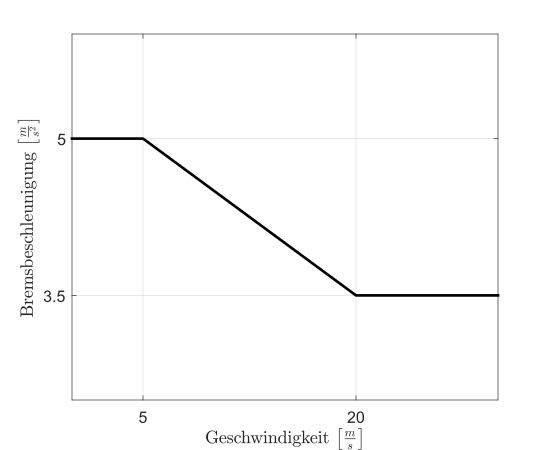
\includegraphics[width=\textwidth]{figures/3_Implementierung/max_acceleration.pdf}
        \caption{maximale Beschleunigung}
        \label{fig:max_acceleration}
    \end{subfigure}
    \hfill
    \begin{subfigure}[b]{.4\textwidth}
        \centering
        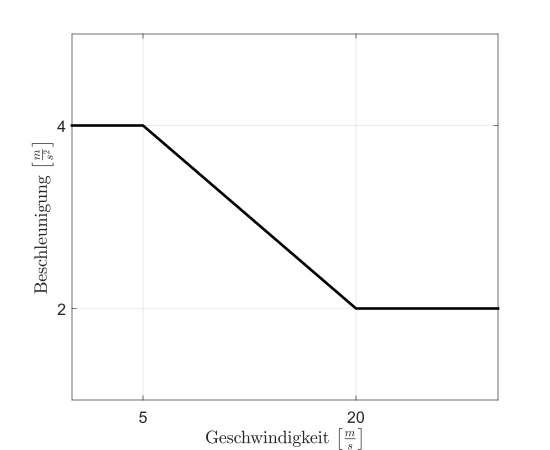
\includegraphics[width=\textwidth]{figures/3_Implementierung/max_deceleration.pdf}
        \caption{maximale Bremsbeschleunigung}
        \label{fig:max_deceleration}
    \end{subfigure}
    \hspace*{\fill}
    \caption{maximal zulässige longitudinale Beschleunigung, Durchschnitt über 2 s \cite{ISO15622}}
    \label{fig:iso_acceleration}
\end{figure}

\bigskip\noindent\textbf{Ruck}

\noindent Ruck ist ein unerwünschtes Verhalten bei Fahrzeugen, das durch ungleichmäßige Beschleunigung und Bremsen entsteht und maßgeblich für den Komfort mitverantwortlich ist. \cite{ISO15622} definiert im ACC Kontext dafür einen Grenzwert für einen negativen longitudinalen Ruck, wie er beim Abbremsen entsteht. Im Kontext dieser Arbeit wird die Bewertung von einem positiven Ruck und der Ruck in lateraler Richtung ähnlich bewertet. In \cite{UNECE_R79} darf der gleitende Mittelwert des lateralen Rucks über eine halbe Sekunde nicht größer als $5\frac{m}{s^{3}}$ sein.
\begin{figure}[ht]
    \centering
    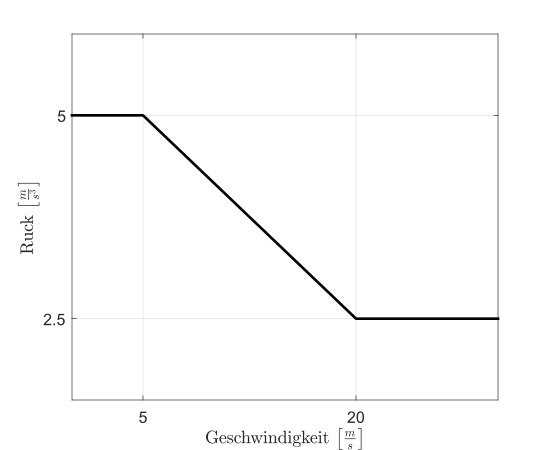
\includegraphics[width=0.4\textwidth]{figures/3_Implementierung/max_neg_jerk.pdf}
    \caption{maximal zulässiger negativer Ruck, Durchschnitt über 1 s \cite{ISO15622}}
    \label{fig:neg_jerk}
\end{figure}

\bigskip\noindent\textbf{Pfadgeschwindigkeitseinhaltung}

\noindent Die Einhaltung der vorgegebenen Pfadgeschwindigkeit ist aus Sicht der Sicherheit und der Gesetzgebung ein wichtiges Kriterium. Eine Unterschreitung ist hier weniger kritisch zu betrachten. Eine Überschreitung sollte vom System vermieden werden. Im Testkatalog von Euro NCAP bekommt ein System, welches die Geschwindigkeit automatisch anpassen kann, die maximale Punktzahl, wenn es die Geschwindigkeit auf $\pm2\frac{km}{h}$ anpassen kann, bevor die Frontachse des Fahrzeugs eine Zone mit einer niedrigeren Pfadgeschwindigkeit betritt \cite{NCAP2024}. Da die Simulation die Hinterachse als Referenz nutzt und darauf regelt wird dieses Kriterum dahingehend angepasst.

\bigskip\noindent\textbf{Weitere KPIs}

\noindent Neben den oben genannten KPIs, welche in der Literatur gängige Anwendung finden und quantifiziert werden, wurden für die jeweiligen Szenarien Weitere definiert.

\begin{itemize}
    \item \textbf{laterale Ablage} - Abweichung der Fahrzeugposition von dem gewünschten Pfad
    \item \textbf{Einschwingzeit} - benötigte Zeit, bis ein Einschwingvorgang abgeschlossen ist
    \item \textbf{Reaktionszeit} - benötigte Zeit, bei der eine Sprungantwort zum ersten mal die neue Sollgröße erreicht 
    \item \textbf{Differenzgeschwindigkeit} - Geschwindigkeitsdifferenz zwischen Ego-Fahrzeug und dem ACC-Target
    \item \textbf{Distanzfehler} - Abweichung von der gewünschten Distanz zwischen dem Ego und einem Zielobjekt
\end{itemize}

\section{Integration in die GitLab CI Pipeline} \label{sec:CIPipeline}
Für das automatisierte Testen in der Pipeline wird eine .yaml-Datei benötigt \cite{GitLabDoks}. In dieser werden Jobs definiert. Ein Job ist die kleinste Einheit einer Pipeline und definiert eine zu erledigende Aufgabe. Eine Pipeline ist somit eine Ansammlung von zeitgleich gestarteten Jobs. Ein Job besteht mindestens aus der Ausführung eines Skriptes, ähnlich einer Kommandozeilenumgebung. Weiterhin kann definiert werden, wann ein Job gestartet wird und welche Voraussetzungen für diesen geschaffen werden müssen.
Für jede Szenario und Fahrzeugkombination kann ein Job erstellt werden. Ein Job führt zunächst Setup-Skripte aus, damit anschließend Matlab\textsuperscript{\textregistered} über eine Befehlszeileneingabe gestartet werden kann. Der Ablauf ist ähnlich zu dem in Abschnitt \ref{fig:Testskript_Ablauf} beschrieben. Es wird lediglich ein anderes Initialisierungsskript verwendet, um mit den geänderten Gegebenheiten in der Pipeline umzugehen.

\subsection{Darstellung der Pipeline}
Um die Wartung der .yaml-Datei und die Ausführung übersichtlicher zu gestalten wird die Funktionalität von Gitlab ausgenutzt, Jobs in einer Matrix zu parametrisieren. Dabei wird lediglich ein Job für jedes Fahrzeug erstellt. In diesem Job werden über den \textit{matrix} Befehl die gewünschten Szenarien, welche für dieses Fahrzeug abgetestet werden sollen, hinterlegt. Die Pipeline generiert dann automatisch für jede Kombination aus Fahrzeug und Szenario einen eigenen Job an. Durch geeignete Wahl der Testklassennamen ist es zusätzlich möglich in einem Job mehrere Testklassen/Szenarien nacheinander laufen zu lassen. Beispielsweise wird im Job "'test\_Curve"' sowohl ein normales Kurvenfahrtszenario als auch der in Abschnitt \ref{sec:kurveNegativ} vorgestellte Negativtest für eine Kurve ausgeführt. Weiterhin können durch die Verwendung des \textit{parallel} Kennworts mehrere Jobs parallel ablaufen, was die Laufzeit der Pipeline enorm verkürzt. Durch diese Einstellung der Pipeline ergibt sich eine sehr übersichtliche Darstellung im Browser (Abbildung \ref{fig:uebersicht_pipeline}). Aus dieser ist direkt zu entnehmen, welche Szenarios für welches Fahrzeug (Alice, IAVShuttle) ausgeführt wurden und welche Szenarien zu Fehlern geführt haben.
\begin{figure}[ht]
    \centering
    \includegraphics[width=0.6\textwidth]{figures/3_Implementierung/uebersicht_pipeline.png}
    \caption{Darstelllung der Jobs in der Gitlab CI Pipeline im Browser. "'Alice"' und "'IAVShuttle"' sind Codenamen von Prototypenfahrezeugen}
    \label{fig:uebersicht_pipeline}
\end{figure}

\subsection{Darstellung der Testergebnisse}
Nachdem ein Szenario durchlaufen ist, werden die Testergebnisse sowohl in GitLab, als auch in einer PDF-Datei dargestellt. Dieser Testbericht wird als Artefakt des jeweiligen Jobs behalten und kann vom Entwickler herunterladen werden.

Auf der Startseite befindet sich eine Übersicht (Abbildung \ref{fig:testreport_aufmacher}). Schlägt ein Test fehl gibt es einen ausführlicheren Bericht (Abbildung \ref{fig:failed_test}). Die Testdiagnose teilt dem Entwickler mit, was das Problem ist. Der Vergleich von soll KPI und tatsächlichem Ergebnis folgt darunter. Wenn es für den Test sinnvoll ist wird ebenfalls ein Plot generiert, der den zeitlichen Verlauf von relevanten Größen über die Zeitdauer der Simulation darstellt. Die Parameter des aktuellen Szenarios werden ebenfalls angegeben, um den Test lokal reproduzieren zu können.
\begin{figure}[ht]
    \centering
    \includegraphics[width=0.5\textwidth]{figures/3_Implementierung/testreport_aufmacher.png}
    \caption{Übersichtliche Darstellung der Testergebnisse eines Szenarios auf der ersten Seite des Testberichts}
    \label{fig:testreport_aufmacher}
\end{figure}
\begin{figure}[ht]
    \centering
    \includegraphics[width=\textwidth]{figures/3_Implementierung/failed_test.png}
    \caption{Darstellung eines fehlgeschlagenen Tests im Testbericht. Der Wert der KPI und der tatsächliche Wert werden verglichen. Ein kurzer Text gibt dem Entwickler wieder, was fehlgeschlagen ist. Wenn sinnvoll wird ein Plot mit den relevanten Daten erzeugt. Die Angabe der Simulationsparameter genutzt werden um diese eine Simulation lokal zu wiederholen.}
    \label{fig:failed_test}
\end{figure}